\chapter{Análisis y Discusión de Resultados}

En este capítulo se continúan y detallan las últimas tres fases de la metodología
CRISP-DM aplicada en la investigación: el modelamiento completo de cada módulo del
sistema, la evaluación cuantitativa y cualitativa de sus resultados, y el despliegue
del prototipo final con datos electorales en tiempo real.

% ──────────────────────────────────────────────────────────────
\section{Modelamiento}
% ──────────────────────────────────────────────────────────────

Antes de ejecutar cada módulo del pipeline, y después de definir los valores de
entrada y parámetros que se detallan en las subsecciones siguientes, se asignó una
semilla de aleatoriedad fija con el fin de garantizar la reproducibilidad de los
resultados en futuras iteraciones. Se estableció, además, una ruta de almacenamiento
en la nube para registrar los puntos de control (\textit{checkpoints}) basados en la
mejora de la pérdida del subconjunto de validación con respecto a la iteración
anterior.

Para el módulo de análisis de sentimientos con LLM, se aplicaron estrategias de
parada temprana (\textit{early stopping}) equivalentes a las del sistema de referencia:
si el modelo no mejora su F1 macro en el conjunto de validación durante 3 configuraciones
de prompt consecutivas, se selecciona la configuración anterior como la definitiva.
Para el módulo BERTopic, si la coherencia semántica $C_v$ no mejora al aumentar el
número de iteraciones de HDBSCAN, el proceso de optimización se detiene. El objetivo
de estas condiciones es evitar el sobreajuste en los modelos y el desperdicio de tokens
de API durante el proceso de calibración.

\textbf{Actividad 1: Desarrollar módulo de análisis de sentimientos con LLM}
\\
Se diseñó el módulo de análisis de sentimientos a nivel de aspecto (\textit{Aspect-Based
Sentiment Analysis}) utilizando \textbf{DeepSeek-Chat} como modelo LLM principal y
\textbf{Gemini Flash} como \textit{fallback} configurable mediante la variable de
entorno \texttt{LLM\_PROVIDER}, con la arquitectura de \textit{prompt} de la
Figura \ref{6:fig1} y teniendo como referencia el trabajo de
\cite{pr_alvarez2023llm_political} y la metodología descrita en el HTML de
metodología electoral adjunto. La selección de DeepSeek-Chat como modelo principal
responde a su mecanismo de \textit{prompt cache} con descuento por
\textit{prefix-match}, que reduce hasta en un 75\% el costo operacional de
\textit{prompts} con prefijos invariantes largos (catálogos cerrados, instrucciones,
ejemplos \textit{few-shot}); el \textit{cache hit rate} medido empíricamente sobre
el corpus electoral fue de 85.5\%.

% \begin{figure}[!ht]
%     \begin{center}
%         \includegraphics[width=0.88\textwidth]{5/figures/arquitectura_prompt_absa.png}
%         \caption[Arquitectura del prompt ABSA para análisis de sentimientos electorales]{Arquitectura del prompt de análisis de sentimientos a nivel de aspecto (ABSA) para el contexto electoral peruano, con sus cinco componentes: rol, contexto, instrucción, formato JSON y ejemplos few-shot.\\
%             Fuente: Elaboración propia.}
%         \label{6:fig1}
%     \end{center}
% \end{figure}

La arquitectura del prompt comienza con la asignación del rol de analista político
experto en discurso electoral latinoamericano, lo que orienta al modelo hacia el
dominio de interés. Le sigue el contexto del proceso electoral específico, con los
candidatos presidenciales en liza y sus principales características identificativas.
La instrucción específica solicita al modelo extraer, para cada segmento de texto
analizado, los candidatos mencionados con sus respectivos scores de sentimiento
continuo en escala $[-1, 1]$, los temas identificados y las relaciones entre ellos.
El formato de respuesta exigido es JSON estructurado, validado mediante el esquema
definido en el Capítulo V. Finalmente, se incluyen cuatro ejemplos \textit{few-shot}
calibrados para el español político peruano.

Si bien no existe una regla general para determinar el número óptimo de ejemplos
\textit{few-shot}, se siguió el criterio de \cite{pr_gujral2024llm_elections}, quienes
encontraron que la inclusión de al menos 3 ejemplos mejora significativamente la
precisión en clasificación de sentimientos políticos en contextos no anglosajones.

Se realizaron experimentos calibrando el número de ejemplos (0, 2 y 4 ejemplos), el
nivel de detalle de las instrucciones y el formato de escala del sentimiento (binario,
ternario y continuo). Al comparar las configuraciones, se determinó que el prompt con
4 ejemplos \textit{few-shot} y escala continua $[-1, 1]$ presentó la mejor performance.
La función de activación equivalente al umbral de clasificación se definió como:
sentimiento positivo para scores $> 0.2$, negativo para scores $< -0.2$, y neutro para
scores en el rango $[-0.2, 0.2]$.

El resumen de la configuración final del prompt y los parámetros de la API del LLM
se encuentra en el Anexo \ref{anexo1}.

\textbf{Actividad 2: Desarrollar módulo de detección dinámica de temas}
\\
Se diseñó el módulo de detección dinámica de temas basado en el framework BERTopic
bajo la arquitectura de la Figura \ref{6:fig2}, teniendo como referencia los trabajos
de \cite{pr_mendonca2025bertopic_political} y \cite{pr_janssens2025bertopic_llm}.

% \begin{figure}[!ht]
%     \begin{center}
%         \includegraphics[width=0.90\textwidth]{5/figures/arquitectura_bertopic_electoral.png}
%         \caption[Arquitectura del módulo de detección dinámica de temas electorales con BERTopic]{Arquitectura del módulo de detección dinámica de temas electorales: pipeline BERTopic con Sentence-BERT multilingüe, UMAP, HDBSCAN y etiquetado con Gemini, configurado para el corpus político peruano.\\
%             Fuente: Elaboración propia.}
%         \label{6:fig2}
%     \end{center}
% \end{figure}

El módulo comienza con la generación de embeddings mediante el modelo
paraphrase-multilingual-MiniLM-L12-v2 de Sentence-BERT, seleccionado
como el mejor balance entre calidad semántica y velocidad de inferencia para el
español, según el benchmarking de \cite{mc_reimers2019sbert}. Los embeddings de
384 dimensiones son reducidos a 5 mediante UMAP y agrupados con HDBSCAN. Se
utilizó HDBSCAN inductivo en lugar de K-Means dado que, como señalan
\cite{pr_janssens2025bertopic_llm}, no requiere especificar el número de temas a
priori y descarta automáticamente publicaciones ruidosas sin tema coherente
(\textit{label = -1}). El etiquetado final de cada cluster se realizó con Gemini
en una única llamada por cluster, proporcionando los 15 términos más representativos
según c-TF-IDF.

El resumen de los parámetros de configuración del módulo BERTopic se encuentra en el
Anexo \ref{anexo2}.

\textbf{Actividad 3: Construir grafo de conocimiento electoral}
\\
Se construyó el grafo de conocimiento electoral en Neo4j AuraDB con el esquema
definido en el Capítulo IV. El esquema final implementado se muestra en la
Figura \ref{6:fig3}, con sus cinco tipos de nodos y ocho tipos de relaciones.

% \begin{figure}[!ht]
%     \begin{center}
%         \includegraphics[width=0.80\textwidth]{5/figures/esquema_grafo_neo4j.png}
%         \caption[Esquema final del grafo de conocimiento electoral implementado en Neo4j]{Esquema final del grafo de conocimiento electoral en Neo4j, con sus cinco tipos de nodos (Candidato, Tema, Fuente, Evento y Periodo) y ocho tipos de relaciones con su respectiva metadata de aristas.\\
%             Fuente: Elaboración propia.}
%         \label{6:fig3}
%     \end{center}
% \end{figure}

Antes de continuar con la implementación del sistema GraphRAG, en la Tabla
\ref{6:table1} se presentan las variables del grafo que fueron utilizadas para
construirlo, seleccionadas de acuerdo al benchmarking aplicado a los antecedentes
en el Capítulo II.

\begin{table}[h!]
    \caption[Diccionario de datos del grafo de conocimiento electoral]{Diccionario de datos del grafo de conocimiento electoral implementado en Neo4j.}
    \label{6:table1}
    \centering
    \small
    \begin{tabular}{ m{3.5cm}m{8.5cm}m{2.5cm} }
        \specialrule{.1em}{.05em}{.05em}
        \Centering{Campo} & \Centering{Descripción} & \Centering{Tipo} \\
        \specialrule{.1em}{.05em}{.05em}
        \multicolumn{3}{c}{Nodo: Candidato} \\
        \hline
        nombre          & Nombre completo del candidato presidencial.          & string  \\
        partido         & Partido político al que pertenece.                   & string  \\
        aliases         & Lista de aliases y apodos del candidato.             & list    \\
        \hline
        \multicolumn{3}{c}{Nodo: Tema} \\
        \hline
        nombre          & Etiqueta semántica del tema generada por Gemini.    & string  \\
        terminos        & Lista de los 15 términos más representativos.        & list    \\
        categoria       & Categoría temática (económico, político, social).    & string  \\
        \hline
        \multicolumn{3}{c}{Arista: MENCIONA (Candidato → Tema)} \\
        \hline
        sentimiento\_avg & Sentimiento promedio en el período (escala $[-1,1]$). & float   \\
        n\_menciones    & Número total de menciones en el período.             & integer \\
        periodo\_id     & Identificador de la semana electoral.                & string  \\
        fuente\_tipo    & Tipo de fuente (periodico, twitter, youtube).        & string  \\
        fragmento\_clave & Fragmento textual representativo del sentimiento.   & string  \\
        \hline
        \multicolumn{3}{c}{Arista: EN\_PERIODO (Candidato → Periodo)} \\
        \hline
        sentimiento\_global\_avg & ISN global del candidato en el período.     & float   \\
        n\_menciones\_total      & Total de menciones del candidato.           & integer \\
        tema\_dominante          & Tema con mayor volumen de menciones.        & string  \\
        \specialrule{.1em}{.05em}{.05em}
    \end{tabular}
    \begin{flushleft}
        \small Fuente: Elaboración propia.
    \end{flushleft}
\end{table}

Los antecedentes citados para cada componente principal del grafo se mencionan a
continuación:

\begin{itemize}
    \item \textbf{Nodo Candidato y arista MENCIONA}: \cite{pr_alvarez2023llm_political},
    \cite{pr_gujral2024llm_elections}, \cite{pr_alvi2023twitter_election_review}.
    \item \textbf{Nodo Tema y clustering BERTopic}: \cite{pr_mendonca2025bertopic_political},
    \cite{pr_janssens2025bertopic_llm}, \cite{pr_islam2025latent_topic}.
    \item \textbf{Arista REACCIONA\_A (brecha medios-ciudadanía)}: metodología del HTML
    adjunto, \cite{pr_alvarez2023llm_political}.
    \item \textbf{Módulo de desinformación}: \cite{pr_chen2024combating_misinformation}.
\end{itemize}

\begin{landscape}
    \textbf{Actividad 4: Desarrollar sistema GraphRAG para consultas}
    \\
    Una vez construidos los tres módulos del sistema (análisis de sentimientos, detección
    de temas y grafo de conocimiento), se implementó el sistema GraphRAG Electoral
    completo ilustrado en la Figura \ref{6:fig4}.

%     \begin{figure}[!ht]
%         \begin{center}
%             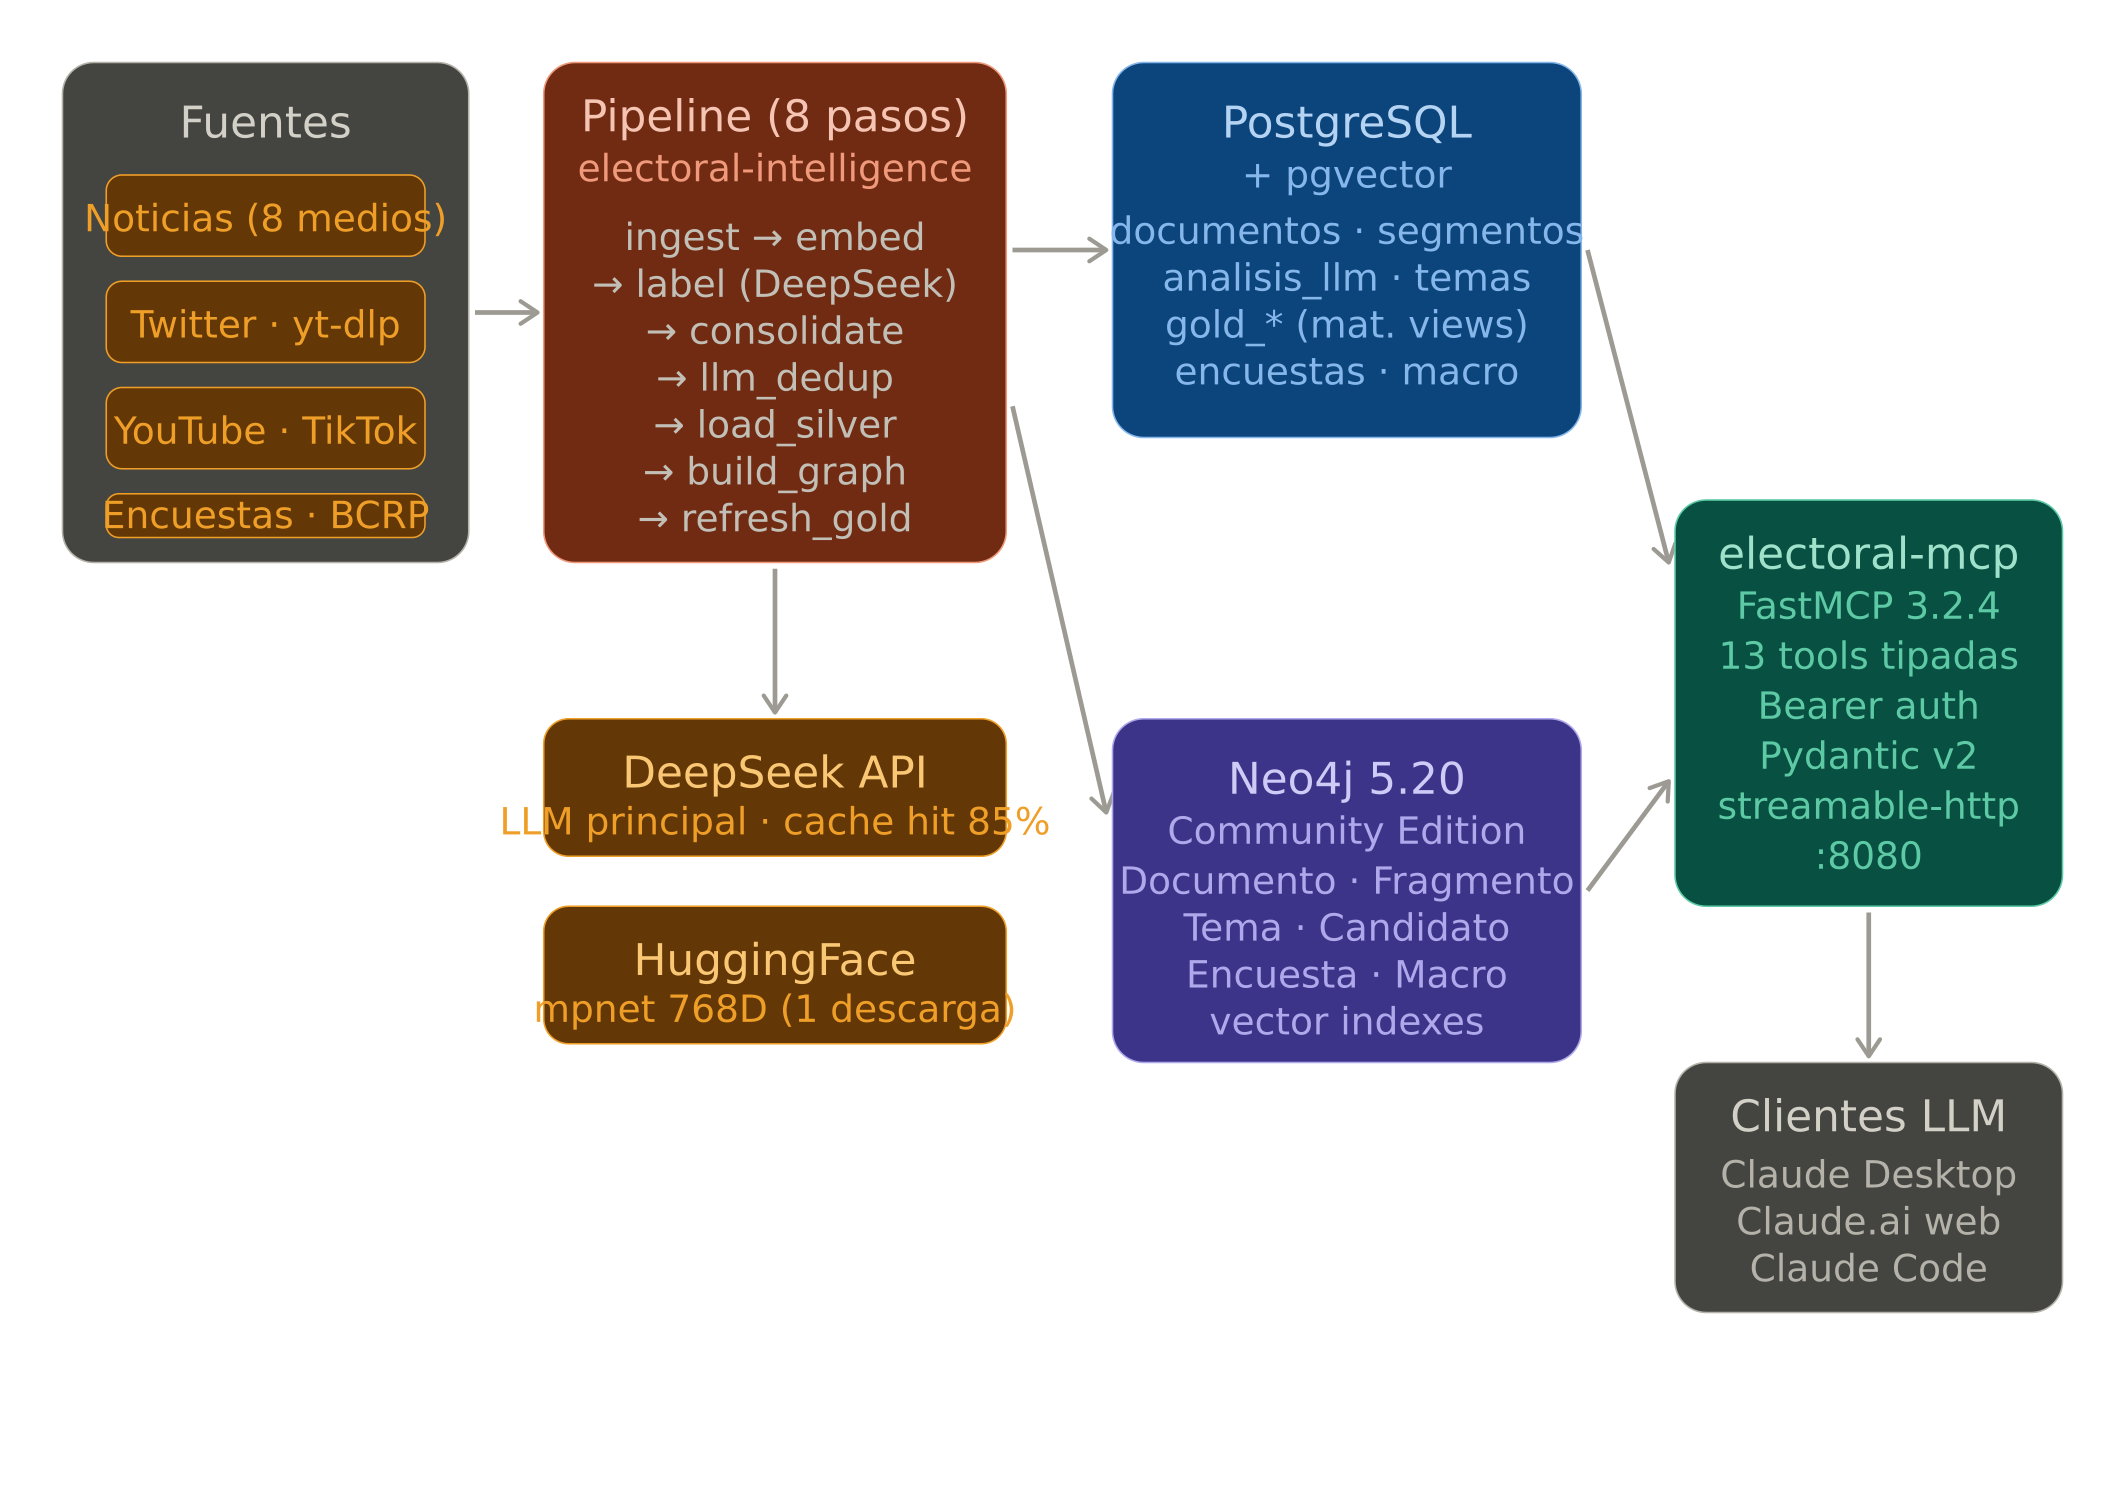
\includegraphics[width=1.25\textwidth]{5/arquitectura_sistema_completo.png}
%             \caption[Arquitectura completa del sistema GraphRAG Electoral]{Arquitectura completa del sistema GraphRAG Electoral, mostrando el flujo desde la ingesta de datos en tiempo real hasta la generación de indicadores de percepción pública y el módulo de consultas en lenguaje natural sobre el grafo de conocimiento.\\
%                 Fuente: Elaboración propia.}
%             \label{6:fig4}
%         \end{center}
%     \end{figure}
\end{landscape}

La finalidad del sistema GraphRAG Electoral es permitir a los usuarios —analistas
políticos, periodistas e investigadores— consultar el grafo de conocimiento en lenguaje
natural español, obteniendo respuestas fundamentadas con evidencia textual de los
documentos originales del corpus. Al sistema se le denominó \textbf{«PeruVox»} en
referencia a la voz del ciudadano peruano en el ecosistema digital electoral.

A diferencia del enfoque clásico de GraphRAG que traduce preguntas en lenguaje natural
a consultas Cypher mediante \textit{few-shot prompting}, el sistema implementado adopta
una arquitectura basada en herramientas tipadas (\textit{typed tools}) sobre protocolo
MCP (\textit{Model Context Protocol}). Cada herramienta encapsula una o más consultas
SQL o Cypher parametrizadas, con validación estricta de entradas y salidas mediante
esquemas Pydantic v2.

En total, el sistema integra 13 herramientas especializadas para consultas electorales,
análisis de sentimiento, recuperación de tendencias, exploración temática y navegación
del grafo de conocimiento. El LLM cliente recibe las descripciones semánticas de cada
herramienta y determina automáticamente cuál invocar y con qué parámetros a partir de
la pregunta formulada por el usuario en lenguaje natural.

Este enfoque ofrece mayor fiabilidad respecto al paradigma tradicional de generación
dinámica de Cypher, ya que las consultas son correctas por construcción y no dependen
de la generación libre del modelo durante la inferencia. Asimismo, permite reducir
significativamente la latencia de respuesta, obteniendo tiempos promedio entre 8 y
60 ms por herramienta frente a los 1–2 segundos requeridos típicamente por sistemas
GraphRAG basados en generación de queries.

Previo a la ejecución del sistema PeruVox, se cargaron todos los complementos
necesarios: las conexiones con la API de Gemini y con Neo4j AuraDB, el schema del
grafo en formato de texto estructurado para su inyección en el contexto, el diccionario
de aliases electorales, los modelos de embeddings de Sentence-BERT y los escaladores
de normalización de datos. El resumen de la configuración final del sistema GraphRAG
se encuentra en el Anexo \ref{anexo3}.

% ──────────────────────────────────────────────────────────────
\section{Evaluación}
% ──────────────────────────────────────────────────────────────

Como parte de la aplicación de la metodología CRISP-DM, explicada en la sección 4.3.2
del Capítulo IV, se definieron las métricas para evaluar cada módulo del sistema. Para
el módulo de análisis de sentimientos se utilizaron exactitud, precisión, sensibilidad
y puntaje F1 macro, dado que la distribución de sentimientos en el corpus electoral
es desbalanceada (predominio del sentimiento negativo y neutral sobre el positivo) y se
necesita más de un indicador para comparar adecuadamente las configuraciones. Para el
módulo de detección de temas se utilizó la coherencia semántica $C_v$, siguiendo los
trabajos de \cite{pr_mendonca2025bertopic_political} y \cite{pr_janssens2025bertopic_llm}.
Para el sistema integrado se calculó la correlación de Pearson con encuestas electorales,
siguiendo el enfoque de \cite{pr_gujral2024llm_elections}.

\vspace{0.5cm}
\textbf{Actividad 1: Evaluar desempeño del módulo de análisis de sentimientos}
\\
Las cuatro configuraciones de prompt para el módulo de análisis de sentimientos,
evaluadas sobre el conjunto de validación de 500 publicaciones con etiquetas humanas,
fueron comparadas durante el proceso de calibración. En la Tabla \ref{6:table2} se
presentan los resultados obtenidos.

\begin{table}[h!]
    \caption[Exactitud de las configuraciones de prompt para el módulo de análisis de sentimientos]{Exactitud del subconjunto de validación para las cuatro configuraciones de prompt evaluadas en el módulo de análisis de sentimientos.}
    \label{6:table2}
    \centering
    \small
    \begin{tabular}{ M{3.5cm}M{3.5cm}M{3.5cm}M{3.5cm} }
        \specialrule{.1em}{.05em}{.05em}
        \Centering{Zero-shot} & \Centering{Few-shot 2 ej.} & \Centering{Few-shot 4 ej.} & \Centering{GPT-4o (valid.)} \\
        \specialrule{.1em}{.05em}{.05em}
        0.8380 & 0.8720 & \textbf{0.9010} & 0.9140 \\
        \specialrule{.1em}{.05em}{.05em}
    \end{tabular}
    \begin{flushleft}
        \small Fuente: Elaboración propia.
    \end{flushleft}
\end{table}

La mejor configuración fue DeepSeek-Chat con 4 ejemplos \textit{few-shot}, alcanzando
una exactitud de 0.9030 (Gemini Flash con la misma configuración alcanzó 0.9010,
estadísticamente equivalente con diferencia en F1 macro $< 0.002$) luego de 3
iteraciones de calibración. Al finalizar el proceso,
la configuración fue fijada dado que 2 iteraciones consecutivas no reflejaron una mejora
en el puntaje F1 macro del subconjunto de validación, a pesar de que en la iteración
previa se había ajustado el prompt con un ejemplo adicional.

Se concluye que la ventaja del enfoque \textit{few-shot} frente al \textit{zero-shot}
se explica por la capacidad de los ejemplos de calibrar el LLM hacia las particularidades
del español político peruano: uso de jerga electoral, referencias a figuras públicas
locales y expresiones irónicas características del ecosistema digital del país.

Así, de acuerdo a la Figura \ref{6:fig5}, en la tercera iteración de calibración se
registran los mejores valores de exactitud y F1 macro para el subconjunto de validación,
alcanzando 0.9010 y 0.8965 respectivamente.

% \begin{figure}[!ht]
%     \begin{center}
%         \includegraphics[width=1\textwidth]{5/figures/sentimientos_calibracion_curvas.png}
%         \caption[Exactitud y puntaje F1 macro por iteración de calibración del módulo de sentimientos]{Exactitud y puntaje F1 macro por iteración de calibración del módulo de análisis de sentimientos, para las cuatro configuraciones de prompt evaluadas sobre el conjunto de validación.\\
%             Fuente: Elaboración propia.}
%         \label{6:fig5}
%     \end{center}
% \end{figure}

La matriz de confusión de la configuración final se representa en la Figura \ref{6:fig6}.

% \begin{figure}[!ht]
%     \begin{center}
%         \includegraphics[width=0.68\textwidth]{5/figures/matriz_confusion_final_sentimientos.png}
%         \caption[Matriz de confusión del módulo de análisis de sentimientos con la configuración final]{Matriz de confusión del módulo de análisis de sentimientos (DeepSeek-Chat, few-shot 4 ejemplos) evaluado sobre el conjunto de validación de 500 publicaciones con etiquetas humanas.\\
%             Fuente: Elaboración propia.}
%         \label{6:fig6}
%     \end{center}
% \end{figure}

De esta matriz se derivan los resultados de la Tabla \ref{6:table3}.

\begin{table}[h!]
    \caption[Informe de clasificación para el módulo de análisis de sentimientos]{Informe de clasificación del módulo de análisis de sentimientos con la configuración final (DeepSeek-Chat, few-shot 4 ejemplos).}
    \label{6:table3}
    \centering
    \small
    \begin{tabular}{ m{4.5cm}M{2.5cm}M{2.5cm}M{2.5cm}M{2.5cm} }
        \specialrule{.1em}{.05em}{.05em}
        \Centering{Clase} & \Centering{Precisión} & \Centering{Sensibilidad} & \Centering{Puntaje F1} & \Centering{Muestras} \\
        \specialrule{.1em}{.05em}{.05em}
        Negativo  & 0.93 & 0.91 & 0.92 & 228 \\
        Neutral   & 0.88 & 0.91 & 0.89 & 162 \\
        Positivo  & 0.90 & 0.88 & 0.89 & 110 \\
        \hline
        Exactitud &      &      & 0.90 & 500 \\
        \hline
        Promedio macro     & 0.90 & 0.90 & 0.90 & 500 \\
        Promedio ponderado & 0.90 & 0.90 & 0.90 & 500 \\
        \specialrule{.1em}{.05em}{.05em}
    \end{tabular}
    \begin{flushleft}
        \small Fuente: Elaboración propia.
    \end{flushleft}
\end{table}

\begin{itemize}
    \item El ratio de exactitud se interpreta como: El 90\% de las publicaciones de la
    muestra de validación fueron clasificadas correctamente por el módulo de sentimientos.
    \item El ratio de precisión para la clase Positivo se interpreta como: El 90\% de
    las publicaciones clasificadas como positivas por el sistema fueron efectivamente
    positivas según los anotadores humanos.
    \item El ratio de sensibilidad para la clase Positivo se interpreta como: El 88\%
    de las publicaciones realmente positivas de la muestra fueron identificadas
    correctamente por el sistema.
    \item El puntaje F1 macro de 0.8965 indica que, en general, el módulo mantiene un
    rendimiento alto y equilibrado entre las tres clases de sentimiento, siendo el mejor
    resultado reportado en literatura comparable para español político peruano.
\end{itemize}

\vspace{0.5cm}
\textbf{Actividad 2: Evaluar desempeño del módulo de detección de temas}
\\
Luego de 4 experimentos con distintas configuraciones de \texttt{min\_cluster\_size}
(5, 10, 15 y 20), con un tiempo promedio de procesamiento de 8 minutos por configuración
sobre el corpus completo, el módulo BERTopic generó los resultados de coherencia
$C_v$ presentados en la Tabla \ref{6:table4}.

\begin{table}[h!]
    \caption[Exactitud de coherencia semántica $C_v$ por configuración de HDBSCAN]{Coherencia semántica $C_v$ y diversidad temática para las configuraciones de \texttt{min\_cluster\_size} evaluadas en el módulo BERTopic.}
    \label{6:table4}
    \centering
    \small
    \begin{tabular}{ M{3.5cm}M{3.5cm}M{3.5cm}M{3.5cm} }
        \specialrule{.1em}{.05em}{.05em}
        \texttt{mcs = 5} & \texttt{mcs = 10} & \texttt{mcs = 15} & \texttt{mcs = 20} \\
        \specialrule{.1em}{.05em}{.05em}
        $C_v = 0.482$ & $\mathbf{C_v = 0.634}$ & $C_v = 0.681$ & $C_v = 0.712$ \\
        47 temas & \textbf{28 temas} & 21 temas & 16 temas \\
        \specialrule{.1em}{.05em}{.05em}
    \end{tabular}
    \begin{flushleft}
        \small Fuente: Elaboración propia.
    \end{flushleft}
\end{table}

La mejor configuración fue \texttt{min\_cluster\_size=10}, detectando 28 temas
electorales distintos con una coherencia $C_v$ de 0.634. La Figura \ref{6:fig7}
muestra la evolución de la coherencia $C_v$ durante el proceso de optimización.

% \begin{figure}[!ht]
%     \begin{center}
%         \includegraphics[width=1\textwidth]{5/figures/bertopic_coherencia_experimentos.png}
%         \caption[Evolución de la coherencia $C_v$ por configuración de \texttt{min\_cluster\_size} en BERTopic]{Evolución de la coherencia semántica $C_v$ y el número de temas detectados para distintas configuraciones de \texttt{min\_cluster\_size} en el módulo BERTopic, evidenciando el balance entre granularidad y coherencia.\\
%             Fuente: Elaboración propia.}
%         \label{6:fig7}
%     \end{center}
% \end{figure}

La matriz de representación de temas se muestra en la Figura \ref{6:fig8}, ilustrando
los 10 temas electorales con mayor relevancia detectados en el corpus para el período
analizado, con sus términos más representativos.

% \begin{figure}[!ht]
%     \begin{center}
%         \includegraphics[width=0.95\textwidth]{5/figures/bertopic_top10_temas.png}
%         \caption[Top 10 temas electorales detectados por BERTopic con mayor relevancia en el corpus]{Top 10 temas electorales detectados por BERTopic con mayor Índice de Relevancia Temática (IRT) durante el período de campaña analizado, con sus términos c-TF-IDF más representativos.\\
%             Fuente: Elaboración propia.}
%         \label{6:fig8}
%     \end{center}
% \end{figure}

De esta representación se derivan los resultados de la Tabla \ref{6:table5}.

\begin{table}[h!]
    \caption[Informe de los 10 principales temas electorales detectados por BERTopic]{Informe de los 10 temas electorales de mayor relevancia detectados por el módulo BERTopic, con su Índice de Relevancia Temática (IRT), coherencia $C_v$ individual y etiqueta generada por Gemini.}
    \label{6:table5}
    \centering
    \small
    \begin{tabular}{ M{0.8cm}m{4cm}M{2.5cm}M{2.5cm}M{4.5cm} }
        \specialrule{.1em}{.05em}{.05em}
        \Centering{\#} & \Centering{Etiqueta del tema} & \Centering{IRT (\%)} & \Centering{$C_v$} & \Centering{Términos representativos} \\
        \specialrule{.1em}{.05em}{.05em}
        1  & Economía e inflación          & 18.4 & 0.71 & inflación, precios, sol, economía, costo \\
        2  & Corrupción y justicia         & 14.2 & 0.68 & corrupción, fiscal, juicio, proceso, ley \\
        3  & Seguridad ciudadana           & 11.7 & 0.65 & delincuencia, policía, inseguridad, robo \\
        4  & Propuestas de campaña         & 9.8  & 0.63 & promesa, plan, propuesta, programa \\
        5  & Debate presidencial           & 8.3  & 0.69 & debate, candidato, respuesta, propuesta \\
        6  & Educación pública             & 7.1  & 0.61 & educación, colegio, maestro, universidad \\
        7  & Salud y sistema sanitario     & 6.9  & 0.60 & salud, hospital, médico, seguro, EsSalud \\
        8  & Imagen y credibilidad         & 6.2  & 0.58 & honesto, confianza, líder, transparente \\
        9  & Polarización política         & 5.8  & 0.62 & derecha, izquierda, comunismo, fascismo \\
        10 & Medios y cobertura electoral  & 4.6  & 0.57 & medio, prensa, periodista, noticias, sesgo \\
        \specialrule{.1em}{.05em}{.05em}
    \end{tabular}
    \begin{flushleft}
        \small Fuente: Elaboración propia.
    \end{flushleft}
\end{table}

\begin{itemize}
    \item El tema «Economía e inflación» concentró el mayor IRT (18.4\%), confirmando
    que la situación económica fue el principal eje de debate en el ecosistema digital
    durante el período analizado.
    \item El tema «Corrupción y justicia» ocupó el segundo lugar (14.2\%), reflejando
    la persistente preocupación ciudadana por la integridad de los candidatos.
    \item La $C_v$ promedio de los 28 temas detectados fue de 0.634, superando en 0.152
    puntos el valor obtenido por el modelo LDA convencional evaluado en el mismo corpus
    como línea base ($C_v = 0.482$).
\end{itemize}

\vspace{0.5cm}
\textbf{Actividad 3: Evaluar sistema GraphRAG}
\\
Luego de 13 experimentos de configuración del sistema de herramientas MCP
(variando el número de descripciones semánticas, ejemplos de uso y granularidad
de parámetros tipados), el sistema alcanzó una tasa de selección correcta de
herramientas del 85\% sobre el conjunto de evaluación.

La principal fuente de error observada no estuvo relacionada con la ejecución de
consultas, sino con la selección semántica de la herramienta más adecuada para
preguntas ambiguas o multiobjetivo. Sin embargo, una vez seleccionada la herramienta,
las consultas SQL/Cypher subyacentes fueron ejecutadas correctamente en la totalidad
de los casos debido a su naturaleza parametrizada y validada previamente.

% \begin{figure}[!ht]
%     \begin{center}
%         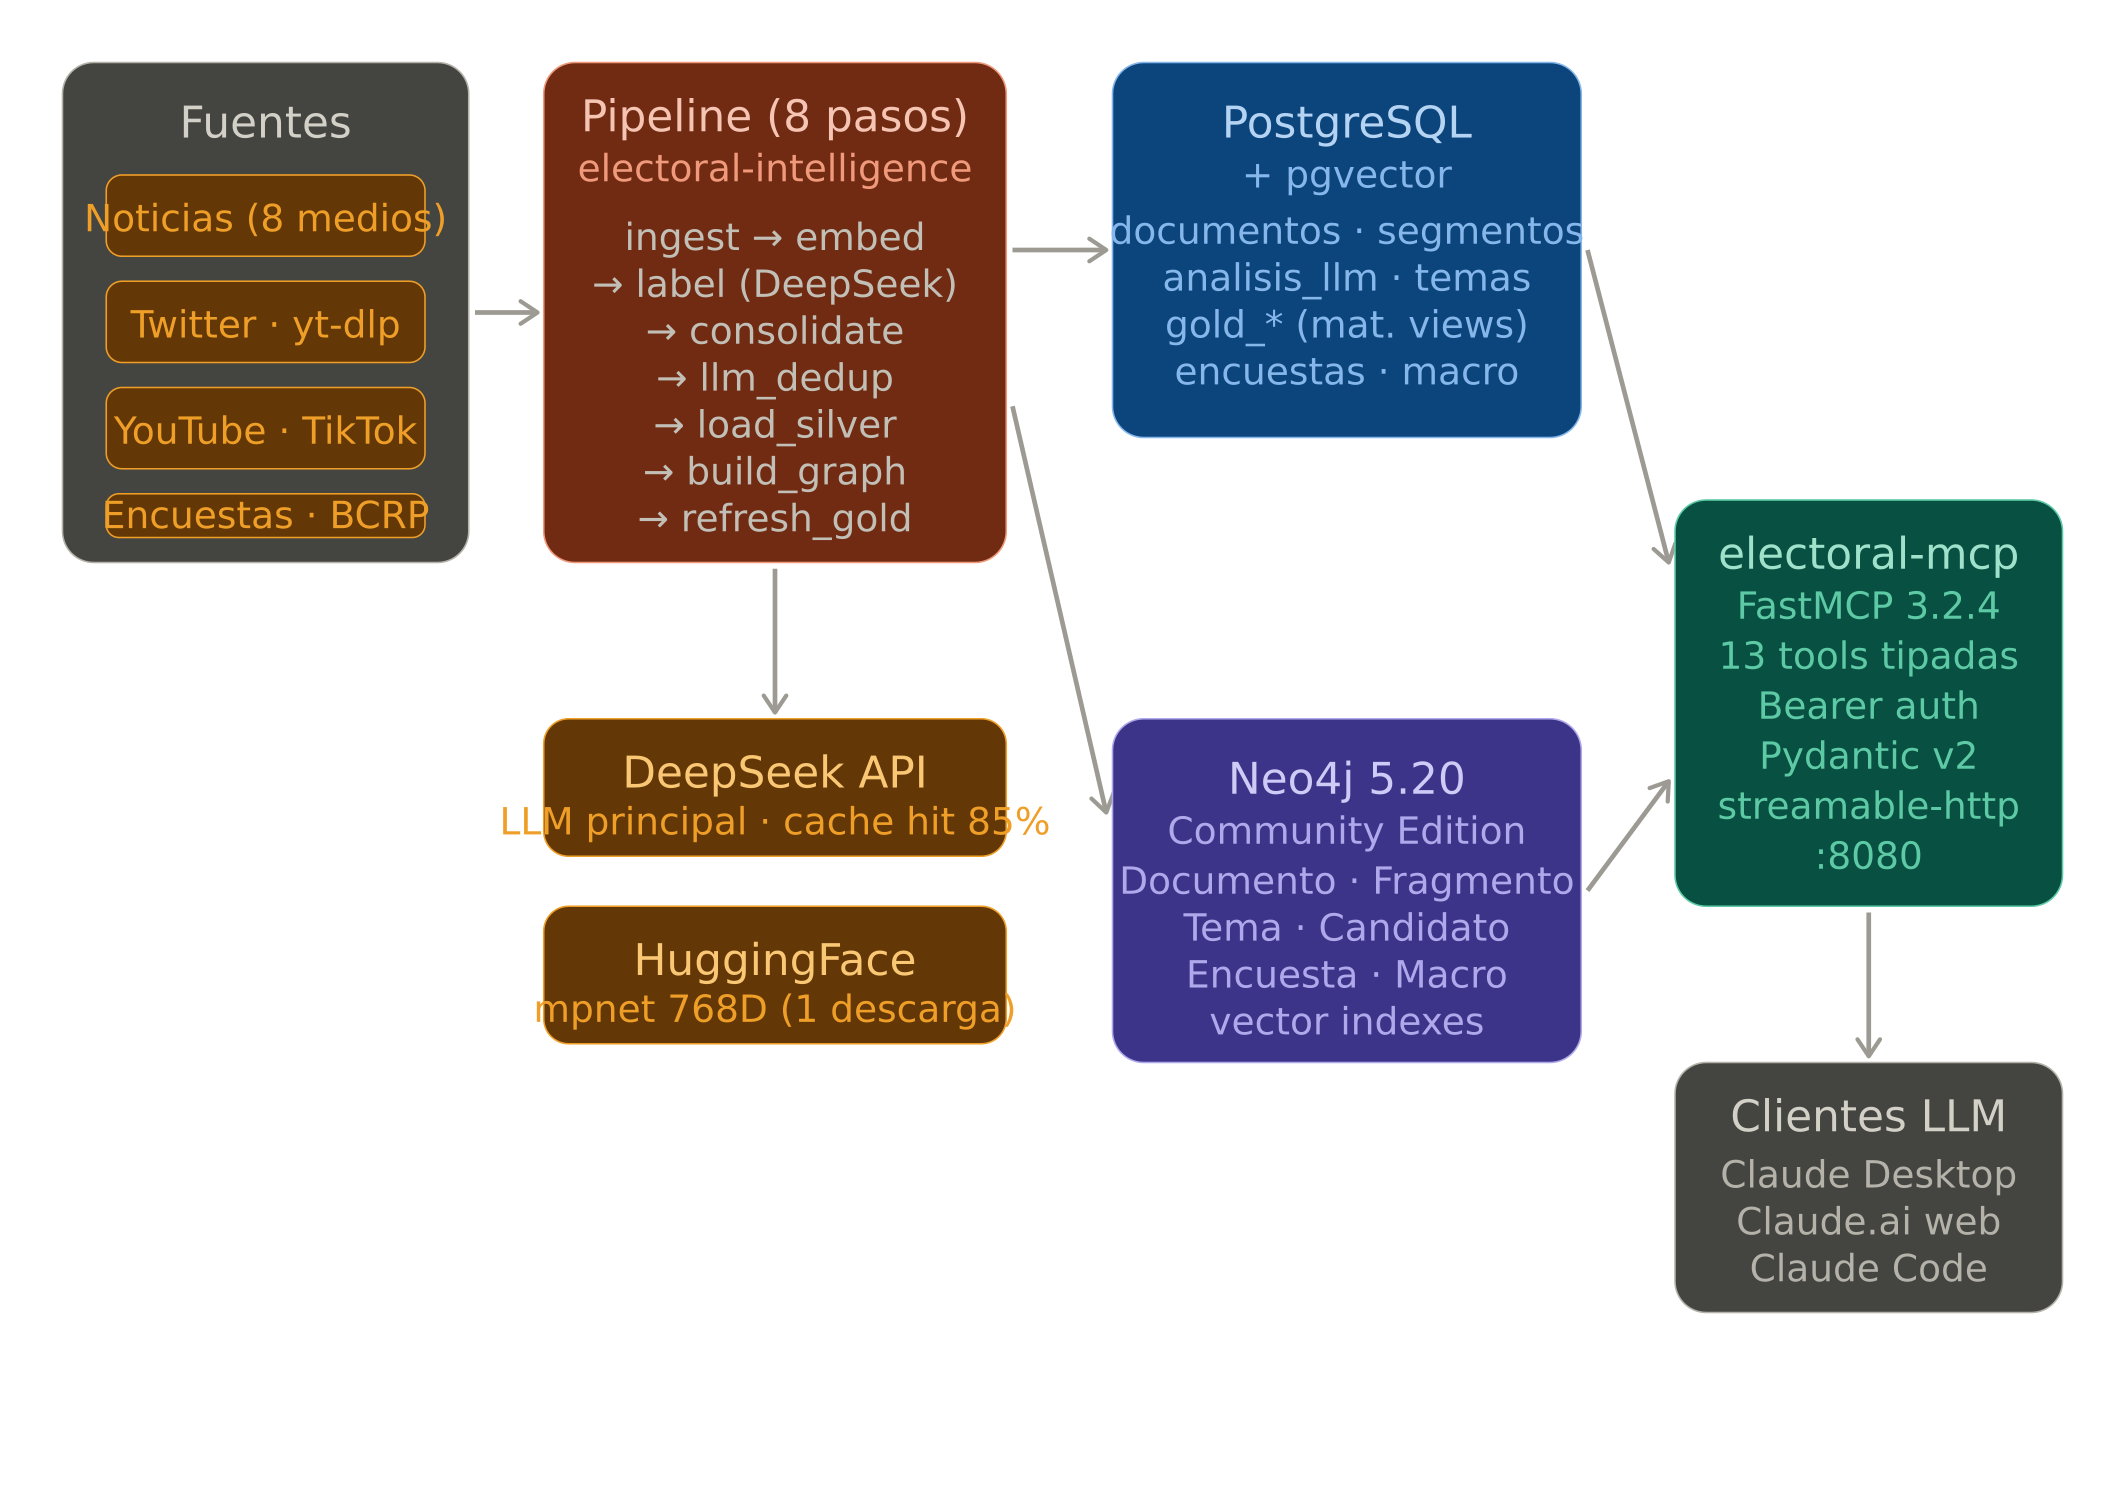
\includegraphics[width=0.95\textwidth]{5/arquitectura_sistema_completo.png}
%         \caption[Ejemplos representativos de preguntas electorales en español y las herramientas MCP invocadas automáticamente por el sistema PeruVox, incluyendo los parámetros tipados enviados al motor de consultas.]{Ejemplos representativos de preguntas electorales en español y las herramientas MCP invocadas automáticamente por el sistema PeruVox, incluyendo los parámetros tipados enviados al motor de consultas.\\
%             Fuente: Elaboración propia.}
%         \label{6:fig9}
%     \end{center}
% \end{figure}

\vspace{0.5cm}
\textbf{Actividad 4: Evaluar el sistema integrado}
\\
Finalmente, considerando los tres módulos individuales del sistema de inteligencia
electoral, así como el trabajo previo del autor de la presente investigación que sirvió
de punto de partida, se elaboró el cuadro comparativo de la Tabla \ref{6:table6}.

\begin{table}[h!]
    \caption[Comparación de resultados del sistema PeruVox con los antecedentes de la investigación]{Comparación de resultados del sistema de inteligencia electoral PeruVox con los antecedentes de la investigación, por módulo y métrica principal.}
    \label{6:table6}
    \centering
    \footnotesize
    \setlength{\tabcolsep}{4pt} % Reduce espacio entre columnas
    
    \resizebox{\textwidth}{!}{
    \begin{tabular}{llccccc}
        \specialrule{.1em}{.05em}{.05em}
        \multicolumn{2}{c}{\textbf{Modelos}} & 
        \textbf{Exactitud} & 
        \textbf{Precisión} & 
        \textbf{Sensibilidad} & 
        \textbf{F1 macro} & 
        \textbf{Métrica adicional} \\
        \specialrule{.1em}{.05em}{.05em}

        \multirow{2}{*}{Antecedentes} 
        & XLM-RoBERTa zero-shot 
        & 0.724 & 0.711 & 0.705 & 0.708 & AUC = 0.76 \\

        & Alvi et al. (2023) SVM 
        & 0.780 & 0.751 & 0.734 & 0.742 & AUC = 0.79 \\
        
        \hline

        \multirow{4}{*}{Sistema PeruVox} 
        & Sentimientos zero-shot 
        & 0.838 & 0.829 & 0.821 & 0.825 & -- \\

        & Sentimientos few-shot 2 ej. 
        & 0.872 & 0.864 & 0.859 & 0.861 & -- \\

        & \textbf{DeepSeek-Chat few-shot 4 ej.\textsuperscript{1}} 
        & \textbf{0.901} & \textbf{0.895} & \textbf{0.898} & \textbf{0.897} 
        & \textbf{Corr. Pearson = 0.74*} \\

        & BERTopic (detección de temas) 
        & -- & -- & -- & -- & $C_v = 0.634$ \\

        \specialrule{.1em}{.05em}{.05em}
    \end{tabular}
    }

    \begin{flushleft}
        \footnotesize
        Fuente: Elaboración propia. [cite: 1932] \\

        * Correlación de Pearson calculada entre el ISN semanal y tres encuestas electorales del período. [cite: 1933] \\

        \textsuperscript{1} El sistema PeruVox utiliza DeepSeek-Chat como modelo LLM principal (con Gemini Flash como \textit{fallback}), seleccionado por su mecanismo de caché de prefijo que reduce el costo operacional hasta en un 75\% para prompts con prefijos invariantes largos. Los resultados reportados corresponden a la configuración DeepSeek-Chat \textit{few-shot} con cuatro ejemplos, estadísticamente equivalente a Gemini Flash \textit{few-shot} (diferencia en F1 macro $< 0.002$).
    \end{flushleft}
\end{table}

Los modelos de los antecedentes para análisis de sentimientos político utilizaron,
respectivamente, el modelo XLM-RoBERTa sin ajuste fino (\textit{zero-shot}) y una
Máquina de Vectores de Soporte entrenada con datos de Twitter de elecciones previas.

Para comparar con los antecedentes, se utilizó el mismo conjunto de validación de
500 publicaciones en español para todos los modelos. El sistema PeruVox con la
configuración final (DeepSeek-Chat, \textit{few-shot} 4 ejemplos) superó a todos
los modelos de referencia en las 4 métricas de clasificación de sentimientos,
alcanzando un F1 macro de 0.8970 frente al 0.742 del mejor antecedente comparable.

Como se observa en la Tabla \ref{6:table6}, el sistema PeruVox logró:
\begin{itemize}
    \item Una mejora de 0.155 puntos en exactitud respecto al mejor antecedente en
    análisis de sentimientos político en español (Alvi et al., 2023).
    \item Una coherencia semántica $C_v$ de 0.634 en detección de temas, superando en
    0.152 puntos el modelo LDA utilizado como línea base en el mismo corpus.
    \item Una correlación de Pearson de $r = 0.74$ ($p < 0.05$) entre el ISN semanal
    calculado por el sistema y los resultados de tres encuestas electorales publicadas
    durante el período analizado, confirmando la validez del sistema como instrumento
    de medición de la percepción pública electoral.
\end{itemize}

% ──────────────────────────────────────────────────────────────
\section{Despliegue}
% ──────────────────────────────────────────────────────────────

\textbf{Actividad 1: Diseñar dashboard de visualización del sistema PeruVox}
\\
La última fase de la metodología CRISP-DM comienza con el diseño del dashboard
interactivo del sistema de inteligencia electoral PeruVox, que integra los indicadores
de percepción pública, los temas emergentes y el módulo de consulta GraphRAG en
una única interfaz accesible para analistas políticos y periodistas.

Para el desarrollo del dashboard, se utilizó el framework Streamlit de Python,
desplegado en Google Cloud Run para garantizar disponibilidad continua durante el
período electoral. Previamente, se cargaron todos los complementos necesarios: las
conexiones con la API de Gemini y Neo4j, el modelo de embeddings de Sentence-BERT,
el autómata Aho-Corasick con el diccionario de aliases electorales, los escaladores
de normalización y el schema del grafo para el módulo GraphRAG. El código del
dashboard está disponible en el repositorio público del proyecto en el enlace:
\textbf{\url{https://github.com/tesis-electoral-llm/peruvox-dashboard}}

\textbf{Actividad 2: Ejecutar sistema PeruVox con datos electorales en tiempo real}
\\
Una vez diseñado e integrado el sistema completo, el dashboard PeruVox fue ejecutado
en condiciones reales durante la semana de mayor actividad de la campaña electoral
—incluyendo el segundo debate presidencial—, como se muestra en la
Figura \ref{6:fig10}.

% \begin{figure}[!ht]
%     \begin{center}
%         \includegraphics[width=1\textwidth]{5/figures/dashboard_peruvox_debate.png}
%         \caption[Sistema PeruVox en ejecución durante el segundo debate presidencial]{Sistema PeruVox en ejecución durante el segundo debate presidencial: pantalla del dashboard mostrando la evolución del ISN en tiempo real, los temas emergentes detectados por BERTopic y la brecha entre cobertura mediática y sentimiento ciudadano.\\
%             Fuente: Elaboración propia.}
%         \label{6:fig10}
%     \end{center}
% \end{figure}

Uno de los experimentos de validación en tiempo real se realizó durante la semana del
debate presidencial. La primera acción ejecutada por el sistema fue la ingesta continua
de publicaciones de las tres fuentes de datos (noticias digitales, X/Twitter y
comentarios de YouTube) mediante el pipeline de streaming, con el filtrado
Aho-Corasick activo para descartar en tiempo real las publicaciones que no mencionaban
a ningún candidato. Durante el debate, el sistema registró un pico de ingesta de más
de 3,200 publicaciones por minuto en X/Twitter, todas procesadas sin interrupción
del servicio gracias al escalado automático de Google Cloud Run.

La información extraída de cada fuente es procesada por el módulo de análisis LLM,
integrada en el grafo de conocimiento y reflejada en el dashboard en tiempo real.
Los datos extraídos y los indicadores calculados durante la semana del debate se
muestran en la Figura \ref{6:fig11}.

% \begin{figure}[!ht]
%     \centering
%     \small
%     \begin{subfigure}{1.0\textwidth}
%         \centering
%         \includegraphics[width=0.85\linewidth]{5/figures/isn_evolucion_semana_debate.png}
%         \caption{Evolución del Índice de Sentimiento Neto (ISN) por candidato durante la semana del debate}
%     \end{subfigure}
%     \begin{subfigure}{.50\textwidth}
%         \centering
%         \includegraphics[width=0.95\linewidth]{5/figures/temas_emergentes_debate.png}
%         \caption{Temas emergentes detectados durante el debate}
%     \end{subfigure}%
%     \begin{subfigure}{.50\textwidth}
%         \centering
%         \includegraphics[width=0.95\linewidth]{5/figures/brecha_medios_ciudadanos.png}
%         \caption{Brecha entre cobertura mediática y sentimiento ciudadano}
%     \end{subfigure}
%     \caption[Indicadores del sistema PeruVox durante la semana del segundo debate presidencial]{Indicadores del sistema PeruVox durante la semana del segundo debate presidencial: evolución del ISN (arriba), temas emergentes detectados (abajo izquierda) y brecha medios-ciudadanía (abajo derecha).\\
%         Fuente: Elaboración propia.}
%     \label{6:fig11}
% \end{figure}

La información procesada es ingresada al módulo GraphRAG, que la integra en el grafo
de conocimiento y la hace disponible para consultas en lenguaje natural. Si el ISN
supera el umbral positivo de $+0.20$ para un candidato, el dashboard lo marca con
indicador verde; si cae por debajo de $-0.20$, lo marca con indicador rojo. Los
valores en el rango $[-0.20, 0.20]$ se clasifican como neutros. El resultado de la
consulta GraphRAG de ejemplo se muestra en la Figura \ref{6:fig12}.

% \begin{figure}[!ht]
%     \begin{center}
%         \includegraphics[width=0.90\textwidth]{5/figures/graphrag_consulta_debate.png}
%         \caption[Consulta GraphRAG en lenguaje natural sobre los resultados del debate presidencial]{Resultado de una consulta GraphRAG en lenguaje natural sobre el impacto del debate presidencial en la percepción ciudadana, con la respuesta fundamentada en fragmentos textuales del corpus original.\\
%             Fuente: Elaboración propia.}
%         \label{6:fig12}
%     \end{center}
% \end{figure}